\documentclass[letterpaper, 12pt]{article}

\usepackage{geometry}
 \geometry{
 letterpaper,
 total={170mm,257mm},
 left=20mm,
 top=20mm,
 bottom=20mm
 }
\usepackage{graphicx} % Required for inserting images
\usepackage{authblk}
\usepackage{amssymb}
\usepackage{lipsum}
\usepackage{float}
\usepackage{times}
\usepackage{amsmath}
\usepackage[format=plain,
            labelfont={bf,it},
            textfont=it]{caption}
\captionsetup{justification=raggedright,singlelinecheck=false}
\usepackage{ragged2e}
\usepackage{longtable}
\usepackage{comment}
\usepackage{setspace}
\usepackage{fancyhdr}
\usepackage{titlesec}
\usepackage[hyperindex,breaklinks]{hyperref}
\hypersetup{
    colorlinks=true,
    linkcolor=blue,
    filecolor=magenta,      
    urlcolor=blue
    }
% \usepackage{background} % add COSIG logo to page
\usepackage[T1]{fontenc}
\usepackage{helvet}
\renewcommand{\familydefault}{\sfdefault}
\pagenumbering{gobble}
\usepackage[skip=10pt plus1pt, indent=40pt]{parskip}

\titlespacing*{\section}
{0pt}{1.5ex plus 1ex minus .2ex}{1.3ex plus .2ex}

\renewcommand\Authfont{\fontsize{12}{14.4}\selectfont}
\renewcommand\Affilfont{\fontsize{9}{10.8}\itshape}
 
\begin{document}
\flushleft

\includegraphics[width=0.5\textwidth]{img/home/241017_final_logo_mockup.png}

\section*{Nucleotide sequence reagents}
\addcontentsline{toc}{section}{Nucleotide sequence reagents}
\textit{Last updated: 3 April 2025}

Nucleotide sequence reagents, short strands of DNA or RNA, are frequently used in a variety of biomedical experiments. Because the sequence of base pairs that compose a nucleotide sequence reagent are \href{https://doi.org/10.1373/clinchem.2008.112797}{expected to be} specified in articles that use these reagents and because the genomes of most organisms used in these experiments are well-characterized, nucleotide sequence reagents are readily verifiable. In other words, most nucleotide sequence reagents can be fact-checked to ensure that they would work as described.

\textit{Note: Nucleotide sequences are typically written and read from the 5\'{} (``five prime'') end to the 3\'{} (``three prime'') end. This guide follows that convention.}

\subsection*{Types of nucleotide sequence reagents}

\subsubsection*{Polymerase chain reaction (PCR) primers}

PCR is a laboratory technique used to make numerous copies of, or \emph{amplify}, a specific DNA sequence known as the \emph{template} sequence. PCR requires the use of two nucleotide sequence primers, typically called the \emph{forward} primer and \emph{reverse} primer. These primers should map to regions of the template sequence that surround the region that should be amplified (called the \emph{amplicon}) on either side. An amplicon is typically 100 to 300 bp (base pairs) long. The forward primer should map to the template sequence and the reverse primer should map to the reverse complement of the template sequence. This ensures that when bound (or \emph{annealed}) to complementary strands of DNA, the primers' 3\'{} ends are pointed toward one another and enclose the amplicon. There are a number of considerations for optimal primer design:

\textit{Note that different guides, some of which are listed under \textbf{Additional resources} below, will provide different specific recommendations for primer design. Those looking to design PCR primers themselves should consult the manufacturer of their reagents for best results.}

\begin{itemize}
    \setlength\itemsep{-0.5em}
    \item \textbf{Each primer should be 18 - 24 bp long.}
    \item \textbf{Primers should have a \href{https://en.wikipedia.org/wiki/GC-content}{GC content} of 40 - 60\%.} Guanine and cytosine bond with three hydrogen bonds, as opposed to adenine and thymine, which bond with two. As a result, GC bonds are stronger are more difficult to break than AT bonds. Primers must have high enough GC content to ensure strong binding between the primer and the template strand, but not so high that the primer sequence is not unique or complex enough to bind specifically to the template strand.
    \item \textbf{The last five bases at the 3\'{} end of each primer should contain 1-2 GC bases.} This inclusion is known as as \emph{GC clamp}. Some guides recommend both starting and ending each primer sequence with 1-2 G or C base pairs. Including more GC bases than this can impair primer specificity. 
    \item \textbf{The melting temperature between each primer should be between 50 - 60 °C and with 5 °C of the other primer's melting temperature.} Melting temperature ($T_m$) is the temperature at which half of the primers will dissociate from the template strand. Melting temperature in Celsius can be roughly estimated by $T_m = 2(A+T) + 4(G+C)$, although more precise estimates of melting temperature can be obtained with online calculators (like \href{https://www.thermofisher.com/us/en/home/brands/thermo-scientific/molecular-biology/molecular-biology-learning-center/molecular-biology-resource-library/thermo-scientific-web-tools/tm-calculator.html}{Thermo Fisher's}).
    \item \textbf{Primers and primer pairs should not contain complementary regions.} Complementary regions within a primer sequence can cause the primer to form a secondary structure (e.g., a loop), preventing the primer from binding properly. Similarly, complementary sequences on both the forward and reverse primer can cause the primers to bind to each other.
\end{itemize}

If either the forward primer or the reverse primer do not actually target the gene of interest, the primer pair will not work as described.

\begin{figure}[h!tbp]
    \centering
    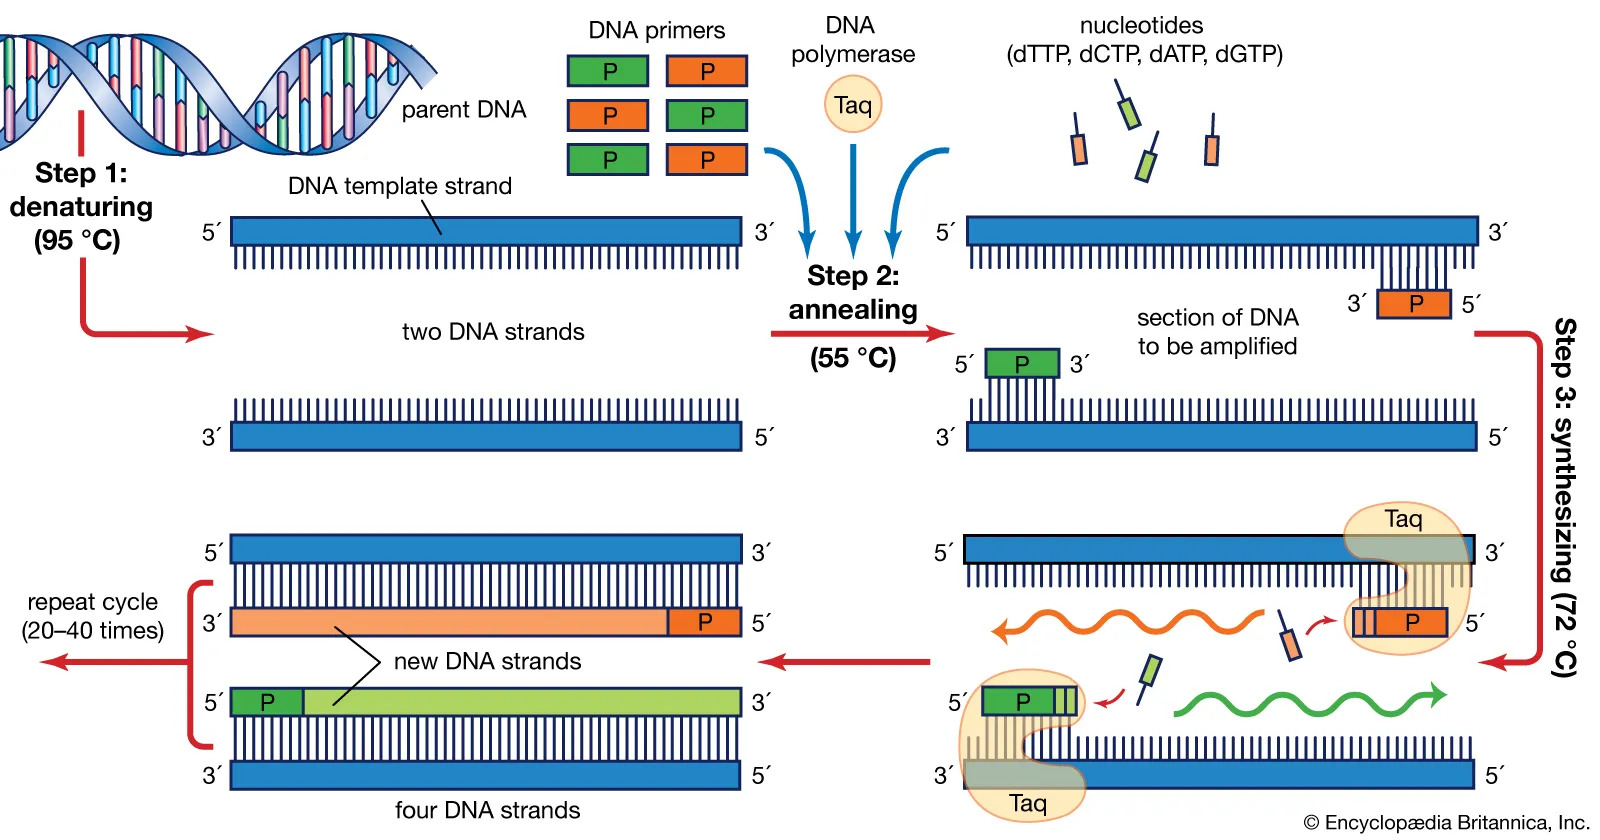
\includegraphics[width=\textwidth]{img/nucleotide_sequences/process-polymerase-chain-reaction.jpg}
    \caption*{Diagram describing the PCR cycle and the role of primers in the synthesis of new DNA strands. From \href{https://www.britannica.com/science/polymerase-chain-reaction}{Encyclop\ae dia Britannica}.}
\end{figure}

\subsubsection*{Revese transcription PCR (RT-PCR) primers}

RT-PCR is used to amplify sections of RNA. More specifically, a \href{https://en.wikipedia.org/wiki/Reverse_transcriptase}{reverse transcriptase} is used to synthesize strands of complementary DNA (\emph{cDNA}) from RNA in a sample and that cDNA is amplified by PCR. Design of RT-PCR primers follows the same principles as design of PCR primers, but the primers should map to a gene's RNA transcripts instead of the DNA genome. To minimize the risk of amplifying contaminating genomic DNA instead of the cDNA of interest, primers should map to regions of the RNA transcript spanning an exon-exon junction or flanking a long intron.

\textit{Note: Reverse transcription PCR should not be confused with real-time PCR, a method for quantifying the amount of a particular DNA molecule in a sample.}

\subsubsection*{Small interfering RNAs (siRNAs) and short hairpin RNAs (shRNAs)}

siRNAs and shRNAs are nucleotide reagents used for RNA interference (\emph{RNAi}). siRNAs are typically double-stranded RNA molecules 18-30 bp long. shRNAs are a single strand of RNA with internally complementary regions (i.e., regions that \emph{hybridize} to one another, forming a \emph{stem-loop structure} where the stem is typically 20-24 bp long and the loop is typically 4-10 bp long. The sequences of siRNAs and the stem region of shRNAs should target unique regions of the transcript of interest. siRNA/shRNA experiments typically use an additional non-targeting sequence (typically one of the targeting sequences with a scrambled sequence) as a negative control. Typically, multiple targeting sequences are used to enhance the efficiency of gene silencing.

\subsection*{Checking nucleotide sequences}

Claimed nucleotide sequences can be checked against the transcripts and genes in the organism of interest using tools like \href{https://blast.ncbi.nlm.nih.gov/Blast.cgi?PROGRAM=blastn}{BLAST} and \href{https://genome.ucsc.edu/cgi-bin/hgBlat}{BLAT}. The tool \href{https://blast.ncbi.nlm.nih.gov/Blast.cgi?PROGRAM=blastn}{Seek \& Blastn} takes a PDF document as input, looks for human nucleotide sequence reagents and BLASTs these sequences against the human genome and transcriptome. The \href{https://dx.doi.org/10.17504/protocols.io.bjhpkj5n}{Seek \& Blastn Standard Operating Procedure} describes how to use this tool in detail. If sequences of interest are not about human genes, skip to Step 5 of this procedure. If the sequences of interest are primers targeting microRNAs, skip to Step 6 of this procedure. If the sequences of interest are RT-PCR primers claiming to target circular RNAs (circRNAs), consult the Methods section of \href{https://doi.org/10.1007/s00210-023-02846-2}{Pathmendra et al. (2024)}.

Tools like BLAST and BLAT take text or files in the \href{https://en.wikipedia.org/wiki/FASTA_format}{.fasta format} as input. This allows multiple sequences to be queried at once. In this format, each entry has a header line (preceded by a `\verb|>|' character) that contains the name of the sequence (note that BLAT does not allow for space characters in the sequence name) and a sequence line containing the sequence. Properly formatted queries are provided in each of the examples below. Try copying these sections into BLAST or BLAT following Step 5 of the \href{https://dx.doi.org/10.17504/protocols.io.bjhpkj5n}{Seek \& Blastn Standard Operating Procedure} to familiarize yourself with these tools. Each of the examples below contain some incorrect sequences and some correct sequences.

\pagebreak

\subsection*{Example 1: Multiple claimed sequences targeting an unrelated gene}

\href{https://doi.org/10.18632/aging.103378}{Dong et al. (2020)} report on experiments involving the gene Nrf2 (standard name \href{https://www.ncbi.nlm.nih.gov/gene/18024}{Nfe2l2}) in models of intestinal ischemia/reperfusion in mouse and human. They provide three PCR primer pairs in their methods section (six sequences in total), not specifying if these primers were used for their experiments in mouse cells or in human cells. These primer sequences are reproduced in .fasta format below.

\begin{verbatim*}
>nrf2_upstream
TAGAGTCAGCAACGTGGAAG
>nrf2_downstream
TATCGAGGCTGTGTCGACTG
>scl7a11_f
GCTGACACTCGTGCTATT
>slc17a11_r
ATTCTGGAGGTCTTTGGT
>ho1_f
TAGAGTCAGCAACGTGGAAG
>ho2_r
TAGAGTCAGCAACGTGGAAG
\end{verbatim*}

Several of these sequences would not be functional as described for mouse or human. \verb|nrf2_upstream| and \verb|nrf2_downstream| do not target \href{https://www.ncbi.nlm.nih.gov/gene/18024}{nrf2/Nfe2l2}. \verb|ho1_f| and \verb|ho1_r| do not target \href{https://www.ncbi.nlm.nih.gov/gene/15368}{HO-1/Hmox1}. Instead, all four sequences appear to target \href{https://www.ncbi.nlm.nih.gov/gene/15251}{Hif1a}. This article was \href{https://doi.org/10.18632/aging.205167}{corrected} in 2023.

\subsection*{Example 2: Claimed non-targeting siRNA sequence targets an unrelated gene}

\href{https://doi.org/10.1016/j.gene.2016.11.046}{Li et al. (2016)} report on experiments involving the gene \href{https://www.ncbi.nlm.nih.gov/gene/11339}{OIP5} in human breast cancer cell lines. They provide two siRNA sequences in the methods section, one claimed to be non-targeting and one claiming to target OIP5. These siRNA sequences are reproduced in .fasta format below.

\begin{verbatim*}
>non_targeting_siRNA
GCCTAACTGTGTCAGAAGGAA
>OIP5_siRNA
ATCAGAGATGGATATTCAA
\end{verbatim*}

\verb|non_targeting_siRNA| should not target any human genes, but instead targets the gene \href{https://www.ncbi.nlm.nih.gov/gene/317781}{DDX51}.

\pagebreak

\subsection*{Example 3: Claimed non-targeting shRNA sequence targets an unrelated gene}

\href{https://doi.org/10.1155/2015/108458}{Lv et al. (2015)} describe experiments involving the non-coding RNA KIAA0125 (standard name \href{https://www.ncbi.nlm.nih.gov/gene/9834}{FAM30A}) in human gallbladder cancer cell lines. They provide two shRNA sequences in the methods section, one targeting KIAA0125 and one non-targeting. These shRNA sequences are reproduced in .fasta format below.

\begin{verbatim*}
>KIAA0125_shRNA
GCAAGGCCAGTGGAGTTAATCCTCGAGGATTAACTCCACTGGCCTTGC
>non_targeting_shRNA
GCGGAGGGTTTGAAAGAATATCTCGAGATATTCTTTCAAACCCTCCGCTTTTTT
\end{verbatim*}

\verb|non_targeting_shRNA| actually targets the gene \href{https://www.ncbi.nlm.nih.gov/gene/7165}{TPD52L2}. This sequence, described by \href{https://doi.org/10.1007/s11192-016-2209-6}{Byrne and Labb\'e (2017)} as `Sequence A', has been used in numerous articles to describe a non-targeting reagent.

\begin{figure}[h!tbp]
    \centering
    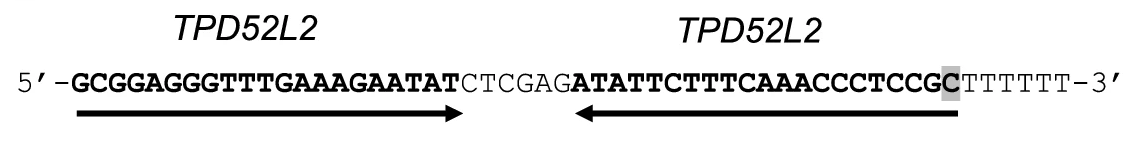
\includegraphics[width=\textwidth]{img/nucleotide_sequences/Screenshot 2025-04-03 at 13-21-09 11192_2021_3871_Fig1_HTML.png}
    \caption*{Diagram showing Sequence A and the regions that target the gene \href{https://www.ncbi.nlm.nih.gov/gene/7165}{TPD52L2}. The nucleotide highlighted in gray is sometimes altered in different versions of the sequence. Adapted from Figure 1 of \href{https://doi.org/10.1007/s11192-021-03871-9}{Byrne et al. (2021)}.}
\end{figure}

\subsection*{Example 4: Multiple claimed RT-PCR primer sequences target unrelated genes in other species}

\href{https://doi.org/10.3892/or.2016.4551}{Lv et al. (2016)} describe experiments related to the gene \href{https://www.ncbi.nlm.nih.gov/gene/10181}{RBM5} in human lung epithelial cells. They provide 18 RT-PCR primer pairs in their methods section (36 sequences in total). A subset of these RT-PCR primer sequences are reproduced in .fasta format below.

\begin{verbatim*}
>CASP3_forward
GAAACCTCCGTGGATTCAAA
>CASP3_reverse
AGCCCATTTCAGGGTAATC
>RBM5_forward
ACACGATGGATGGAAGCCA
>RBM5_reverse
TCTGCTCTGCCTCTGACTT
>VEGF_forward
AAACCCTGAGGGAGGCTC
>VEGF_reverse
TACTTGCAGATGTGACAAGCCG
\end{verbatim*}

\verb|CASP3_forward| and \verb|CASP3_reverse| do not target \href{https://www.ncbi.nlm.nih.gov/gene/836}{CASP3} or any other human gene. Several other RT-PCR primer sequences do not target any gene in humans, instead targeting the claimed gene's counterpart in another species. Instead, they target \href{https://www.ncbi.nlm.nih.gov/gene/25402}{Casp3 in rat}. \verb|RBM5_forward| and \verb|RBM5_reverse| do not target \href{https://www.ncbi.nlm.nih.gov/gene/10181}{RBM5}. Instead, they target \href{https://www.ncbi.nlm.nih.gov/gene/8241}{RBM10}. All wrongly-identified sequences for this article are described in Table S1 of \href{https://doi.org/10.26508/lsa.202101203}{Park et al. (2022)} (Sheet: All sequences, under PMID: 26782095). Some sequences do indeed target the claimed transcript, such as the primer sequences shown above for the gene \href{https://www.ncbi.nlm.nih.gov/gene/7422}{VEGF/VEGFA}.

\subsection*{Additional resources}

\begin{itemize}
    \setlength\itemsep{-0.5em}
    \item \href{https://www.addgene.org/protocols/primer-design/}{AddGene: Primer design for PCR}
    \item \href{https://www.zymoresearch.com/blogs/blog/how-to-design-primers-for-pcr-experiments}{Zymo Research: How to Design Primers for PCR Experiments}
    \item \href{https://www.thermofisher.com/blog/behindthebench/pcr-primer-design-tips/}{Thermo Fisher: PCR Primer Design Tips}
    \item \href{https://sharebiology.com/primer-designing-demonstration-step-by-step/}{Share Biology: Primer Designing – Demonstration step by step}
    \item \href{https://www.thermofisher.com/us/en/home/brands/thermo-scientific/molecular-biology/molecular-biology-learning-center/molecular-biology-resource-library/spotlight-articles/basic-principles-rt-qpcr.html}{Thermo Fisher: Basic principles of RT-qPCR}
    \item \href{https://cellecta.com/pages/principles-of-rnai-and-shrna-design}{Cellecta: Principles of RNAi and shRNA design}
    \item \href{https://doi.org/10.1007/978-1-60761-657-3_10}{``Short Hairpin RNA (shRNA): Design, Delivery, and Assessment of Gene Knockdown'' (2010)}
    \item \href{https://dx.doi.org/10.17504/protocols.io.bjhpkj5n}{Seek \& Blastn Standard Operating Procedure}
    \item \href{https://doi.org/10.1007/s11192-016-2209-6}{``Striking similarities between publications from China describing single gene knockdown experiments in human cancer cell lines'' (2017)}
    \item \href{https://doi.org/10.1371/journal.pone.0213266}{``Semi-automated fact-checking of nucleotide sequence reagents in biomedical research publications: The Seek \& Blastn tool'' (2019)}
    \item \href{https://doi.org/10.1371/journal.pone.0213266}{``Semi-automated fact-checking of nucleotide sequence reagents in biomedical research publications: The Seek \& Blastn tool'' (2019)}
    \item \href{https://doi.org/10.1007/s11192-020-03463-z}{``Flagging incorrect nucleotide sequence reagents in biomedical papers: To what extent does the leading publication format impede automatic error detection?'' (2020)}
    \item \href{https://doi.org/10.1007/s11192-021-03871-9}{``The thin ret(raction) line: biomedical journal responses to incorrect non-targeting nucleotide sequence reagents in human gene knockdown publications'' (2021)}
    \item \href{https://doi.org/10.26508/lsa.202101203}{``Identification of human gene research articles with wrongly identified nucleotide sequences'' (2022)}
    \item \href{https://doi.org/10.1007/s00210-023-02846-2}{``Verification of nucleotide sequence reagent identities in original publications in high impact factor cancer research journals'' (2024)}
\end{itemize}

\end{document}